\documentclass[a4paper,14pt]{extarticle}
\usepackage{../../tex-shared/report-layout}

\renewcommand{\mylabnumber}{4}
\renewcommand{\mylabtitle}{Исследование взаимодействий распределенных процессов типа Клиент-Cервер}
\renewcommand{\mysubject}{Теория распределенных систем и параллельных вычислений}
\renewcommand{\mylecturer}{Дрозин А.Ю.}

\begin{document}
\begin{titlepage}
    
    \thispagestyle{empty}
    
    \begin{center}
        
        Министерство науки и Высшего образования Российской Федерации \\
        Севастопольский государственный университет \\
        Кафедра ИС
        
        \vfill

        Отчет \\
        по лабораторной работе №\mylabnumber \\
        \enquote{\mylabtitle} \\
        по дисциплине \\
        \enquote{\MakeTextUppercase{\mysubject}}

    \end{center}

    \vspace{1cm}

    \noindent\hspace{7.5cm} Выполнил студент группы ИС/б-17-2-о \\
    \null\hspace{7.5cm} Горбенко К. Н. \\
    \null\hspace{7.5cm} Проверил \\
    \null\hspace{7.5cm} \mylecturer

    \vfill

    \begin{center}
        Севастополь \\
        \the\year{}
    \end{center}

\end{titlepage}

\section{Цель работы}
Исследовать механизм взаимодействия распределено выполняющихся параллельных
процессов типа \enquote{клиент-сервер}.

\section{Постановка задачи}
В состав вычислительного кластера входит три хоста, один из которых реализует
функции сервера, два остальных – клиентов. Сервер разграничивает доступ к трем
общим ресурсам – нерешенным, хранящим общую вырученную сумму от продажи товаров,
общее количество товаров и остальных товаров. Доступ к ресурсам осуществляется в
произвольном порядке, все ресурсы разделяются между клиентами по отдельности.
Реализована процедура, выделяющая ресурсы (путем передачи сообщения) в
использование клиентам. Реализовать серверный процесс, который разграничивает
доступ клиентов к этой процедуре (процедурам) и к ресурсам. Реализацию сервера
выполнять в соответствии со схемой управления, использующую рассылку сообщений.


\section{Ход работы}
Текст программы:
\begin{lstlisting}
#include <mpi.h> 
#include <iostream> 
#include <sstream> 
#include <iomanip> 
  
#define CS_CONNECT 0 
#define CS_DISCONNECT 1 
#define CS_TAKE 2 
#define CS_RETURN 3 
  
#define SC_FREE 10 
#define SC_INUSE 11 
#define SC_SET 12 
#define SC_NO_RESOURCE 13 
#define SC_NO_ACTION 14 
  
#define RES_COUNT 3 
  
using namespace std; 
  
void server() { 
    double resources[] = {1234.56, 12, 500}; 
    int inUse[] = {0, 0, 0}; 
  
    bool firstClientConnected = false; 
    int clients = 0, outTag, r_index; 
    double r_value; 
  
    double *inBuf = new double[2]; 
    double *outBuf = new double[1]; 
    MPI_Status status; 
    while (!firstClientConnected || clients) { 
        outBuf[0] = 0; 
        MPI_Recv(inBuf, 2, MPI_DOUBLE, MPI_ANY_SOURCE, MPI_ANY_TAG, MPI_COMM_WORLD, &status); 
        switch (status.MPI_TAG) { 
            case CS_CONNECT: 
                firstClientConnected = true; 
                clients++; 
                break; 
            case CS_DISCONNECT: 
                clients--; 
                break; 
            case CS_TAKE: 
                r_index = (int) inBuf[0]; 
                if (r_index < RES_COUNT) { 
                    if (inUse[r_index] != 0) { 
                        outTag = SC_INUSE; 
                    } else { 
                        outBuf[0] = resources[r_index]; 
                        inUse[r_index] = status.MPI_SOURCE; 
                        outTag = SC_FREE; 
                    } 
                } else { 
                    outTag = SC_NO_RESOURCE; 
                } 
                MPI_Send(outBuf, 1, MPI_DOUBLE, status.MPI_SOURCE, outTag, MPI_COMM_WORLD); 
                break; 
            case CS_RETURN: 
                r_index = (int) inBuf[0]; 
                r_value = inBuf[1]; 
                if (r_index < RES_COUNT) { 
                    if (inUse[r_index] != status.MPI_SOURCE) { 
                        outTag = SC_INUSE; 
                    } else { 
                        resources[r_index] = r_value; 
                        inUse[r_index] = 0; 
                        outTag = SC_SET; 
                    } 
                } else { 
                    outTag = SC_NO_RESOURCE; 
                } 
                MPI_Send(outBuf, 1, MPI_DOUBLE, status.MPI_SOURCE, outTag, MPI_COMM_WORLD); 
                break; 
            default: 
                MPI_Send(outBuf, 1, MPI_DOUBLE, status.MPI_SOURCE, SC_NO_ACTION, MPI_COMM_WORLD); 
        } 
    } 
  
    stringstream ss; 
    ss << "\t" << "Server" << endl; 
    for (r_index = 0; r_index < RES_COUNT; r_index++) { 
        ss << "Resource #" << r_index 
           << " is " << fixed << setw(8) << setprecision(2) << resources[r_index] 
           << endl; 
    } 
    ss << endl; 
    cout << ss.str(); 
  
    delete[] inBuf; 
    delete[] outBuf; 
} 
  
double get_resource(int n) { 
    MPI_Status status; 
    double *inBuf = new double[1]; 
    double *outBuf = new double[1]; 
    outBuf[0] = n; 
    bool received = false; 
    while (!received) { 
        MPI_Send(outBuf, 1, MPI_DOUBLE, 0, CS_TAKE, MPI_COMM_WORLD); 
        MPI_Recv(inBuf, 1, MPI_DOUBLE, 0, MPI_ANY_TAG, MPI_COMM_WORLD, &status); 
        if (status.MPI_TAG == SC_FREE) { 
            received = true; 
        } 
    } 
    double ret_val = inBuf[0]; 
    delete[] inBuf; 
    delete[] outBuf; 
  
    return ret_val; 
} 
  
bool set_resource(int n, double value) { 
    MPI_Status status; 
    double *inBuf = new double[1]; 
    double *outBuf = new double[2]; 
    outBuf[0] = n; 
    outBuf[1] = value; 
    MPI_Send(outBuf, 2, MPI_DOUBLE, 0, CS_RETURN, MPI_COMM_WORLD); 
    MPI_Recv(inBuf, 1, MPI_DOUBLE, 0, MPI_ANY_TAG, MPI_COMM_WORLD, &status); 
  
    delete[] inBuf; 
    delete[] outBuf; 
  
    return status.MPI_TAG == SC_SET; 
} 
  
void client(int rank) { 
    double *outBuf = new double[1]; 
    outBuf[0] = 0; 
    MPI_Send(outBuf, 1, MPI_DOUBLE, 0, CS_CONNECT, MPI_COMM_WORLD); 
  
    stringstream ss; 
    ss << "\t" << "Client #" << rank << endl; 
    double r_value, r_value_changed; 
    for (int r_index = 0; r_index < RES_COUNT; r_index++) { 
        r_value = get_resource(r_index); 
        r_value_changed = r_value + (r_index + 10) * rank; 
        set_resource(r_index, r_value_changed); 
  
        ss << "Resource #" << r_index 
           << " was " << fixed << setw(8) << setprecision(2) << r_value 
           << " set " << fixed << setw(8) << setprecision(2) << r_value_changed 
           << endl; 
    } 
    ss << endl; 
    cout << ss.str(); 
  
    MPI_Send(outBuf, 1, MPI_DOUBLE, 0, CS_DISCONNECT, MPI_COMM_WORLD); 
  
    delete[] outBuf; 
} 
  
int main(int argc, char **argv) { 
    int rank, size; 
    MPI_Init(&argc, &argv); 
    MPI_Comm_size(MPI_COMM_WORLD, &size); 
    MPI_Comm_rank(MPI_COMM_WORLD, &rank); 
    if (size != 3) { 
        if (rank == 0) { 
            cout << "Use only with 3 processes" << endl; 
            cout << "Exit..." << endl; 
        } 
        MPI_Finalize(); 
        return 1; 
    } 
    !rank ? server() : client(rank); 
  
    MPI_Finalize(); 
    return 0; 
}
\end{lstlisting}

На рисунке \ref{fig:result} представлен результат работы программы:
\begin{figure}[H]
    \centering
    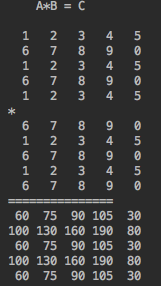
\includegraphics[width=.5\linewidth]{result}
    \caption{Результат работы программы}
    \label{fig:result}
\end{figure}

\section*{Выводы}
В ходе лабораторной работы был исследован механизм взаимодействия распределено
выполняющихся параллельных процессов типа «клиент-сервер».
\end{document}